\documentclass[conference]{IEEEtran}

\usepackage{newtxtext,newtxmath}
\usepackage{amsmath}
\usepackage{booktabs}
\usepackage{graphicx}
\usepackage{longtable}
\usepackage{array}
\usepackage{url}
\usepackage[hidelinks]{hyperref}
\usepackage{tikz}
\usetikzlibrary{arrows.meta}

\urlstyle{tt}
\setlength{\emergencystretch}{3em}
\newcolumntype{L}[1]{>{\raggedright\arraybackslash}p{#1}}
\newcommand{\codepath}[1]{{\Urlmuskip=0mu plus 1mu\relax\nolinkurl{#1}}}

\begin{document}

\title{Geo-Distributed Data Center Demand Scheduling to Reduce Grid Ramps}

\author{\IEEEauthorblockN{Janusz Gal}
\IEEEauthorblockA{jgal@charlotte.edu}}

\maketitle

\begin{IEEEkeywords}
data centers, demand response, grid ramp, net load, reinforcement learning,
workload scheduling
\end{IEEEkeywords}

\section{Introduction and Scope}
\label{sec:introduction}

Large data centers draw enough electrical power that the timing and location of their computing work matters to the grids that serve them. Some work must run immediately, while lower-priority work may be delayed. A
geo-distributed operator may also have more than one site capable of running the same work. These two forms of flexibility create a scheduling question: can computing load be placed where and when it makes regional grid net-load ramps smaller without dropping work or violating service and deadline rules?

The question we ask here is:
\begin{quote}
\emph{Relative to running every job where and when it arrived, how much can a
causal scheduler reduce normalized one-hour and three-hour regional net-load
ramps by jointly using temporal deferral and geographic routing, while
satisfying immediate-service, batch-window, and site-capacity constraints?}
\end{quote}

To do this, we leverage data from a Google data center workload trace and EIA grid and energy data, to create a synthetic four-site data center fleet with real demand and workloads, to optimize.

At the centre of that fleet sits a \emph{hypothetical scheduler}. Every hour it makes two kinds of decision: where the work that must run immediately should run, and how much of the deferrable backlog to release and to which sites. This paper defines that decision problem. It sets out the data the scheduler is given, the constraints it has to respect, and the quantity by which its choices are judged. It does not optimize those choices; that is planned for a later chapter using reinforcement learning (PPO).

Taken as a whole, the thesis will do five things: build a trace-driven synthetic model that joins the workload, data-center power, and balancing-authority grid data; define a causal scheduling environment with hard capacity and completion-window constraints; train a PPO scheduler that uses both temporal and geographic flexibility; compare it against one clearly defined operating policy, running every job where and when it arrived; and check whether the conclusion survives when a small set of the modeling assumptions is varied. This chapter covers the first two.

Note we are specifically targeting net-load ramps rather than electricity cost. What determines how much fast-moving generation an operator must keep available is not the price of power but the rate at which net load changes, so that is the quantity this study works with.

\section{Google ClusterData2019 Workload Trace}
\label{sec:clusterdata2019}

\subsection{Dataset}
\label{subsec:clusterdata-role}

A \emph{Borg cell} is a group of machines managed as one computing cluster.
Google provides records for eight cells, labeled \(a\)--\(h\), from May 2019
\cite{wilkes2020clusterdata2019, tirmazi2020borg}. The trace includes machine
capacity, per-instance resource usage, collection events, priorities, and
resource requests. It is sanitized: it contains no user, application,
location, or other identifying information.

Three tables supply the workload data used here: \codepath{machine_events}
for the CPU reference capacity, \codepath{instance_usage} for measured CPU
execution, and \codepath{collection_events} for
priority.\footnote{The full trace is approximately 2.4 TiB, so the extraction
queries it through BigQuery rather than downloading it.}

One point of clarification worth noting: rather than scheduling individual jobs, we are scheduling  \emph{CPU utilization} (specifically how much of a cell was busy in
each five-minute window, and the fraction that was service/batch demand). A priority split is applied to the utilization itself, so a cell that is 60\% busy with a quarter of that work deferrable becomes 45\% service and 15\% batch, not a list of tasks.

This is a deliberate simplification. While there is data to track requested CPU usage per individual job, the resultant demand we schedule is the same total work being placed at a site. Essentially - we don't carry through which job contributed to what usage, but still deliver the same end usage.  

\begin{figure}[!ht]
  \centering
  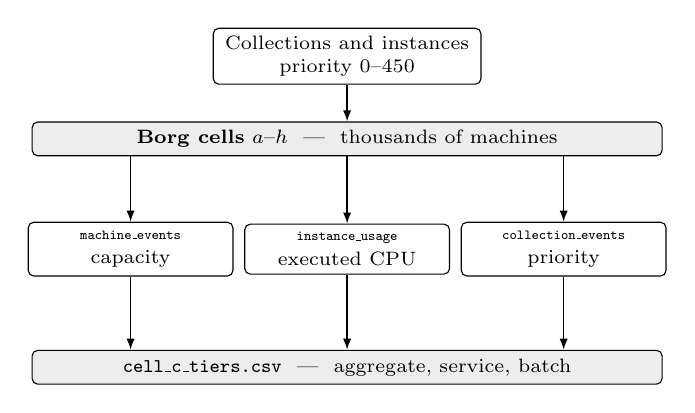
\begin{tikzpicture}[
    font=\scriptsize,
    box/.style={draw, rounded corners=2pt, align=center, inner sep=3pt},
    shaded/.style={box, fill=black!7},
    arr/.style={-{Latex[length=1.4mm]}, semithick}
  ]
    \node[box, minimum width=34mm] (jobs) at (0,0)
      {Collections and instances\\priority 0--450};

    \node[shaded, minimum width=80mm] (cell) at (0,-1.05)
      {\textbf{Borg cells} \(a\)--\(h\)\ \ ---\ \ thousands of machines};

    \node[box, minimum width=26mm] (me) at (-2.75,-2.45)
      {\texttt{\tiny machine\_events}\\[1pt]capacity};
    \node[box, minimum width=26mm] (iu) at (0,-2.45)
      {\texttt{\tiny instance\_usage}\\[1pt]executed CPU};
    \node[box, minimum width=26mm] (ce) at (2.75,-2.45)
      {\texttt{\tiny collection\_events}\\[1pt]priority};

    \node[shaded, minimum width=80mm] (csv) at (0,-3.95)
      {\texttt{cell\_c\_tiers.csv}\ \ ---\ \ aggregate, service, batch};

    \draw[arr] (jobs) -- (cell);
    \draw[arr] (cell.south -| me) -- (me.north);
    \draw[arr] (cell.south -| iu) -- (iu.north);
    \draw[arr] (cell.south -| ce) -- (ce.north);
    \draw[arr] (me.south) -- (me.south |- csv.north);
    \draw[arr] (iu.south) -- (iu.south |- csv.north);
    \draw[arr] (ce.south) -- (ce.south |- csv.north);
  \end{tikzpicture}
  \caption{Extraction path from the Google trace to the retained five-minute
  tier curves. The symbol \(c\) identifies a Google cell.}
  \label{fig:clusterdata-pipeline}
\end{figure}

\subsection{Fixed reference capacity}
\label{subsec:clusterdata-capacity}

Google expresses CPU capacity in normalized units, with the largest machine
equal to 1.0. We then define a cell's reference capacity as the sum over its machines:
\begin{equation}
  C^{\mathrm{ref}}_c
  =
  \sum_{n\in\mathcal{J}_c}\kappa_n ,
  \label{eq:reference-capacity}
\end{equation}
where \(\mathcal{J}_c\) is all machines ever observed in cell \(c\)
and \(\kappa_n\) is machine \(n\)'s largest reported
\codepath{capacity.cpus}.\footnote{A machine can appear more than once in
\codepath{machine_events} because of add, update, and snapshot records; the
largest reported value is kept. Equation~\eqref{eq:reference-capacity} is
therefore a fixed monthly reference rather than the active machine capacity
in each five-minute interval, and this fixed denominator is used throughout.}

\subsection{Five-minute executed CPU}
\label{subsec:clusterdata-utilization}

For every five-minute window, we add up the CPU utilization that actually ran and divide
by the cell's capacity, which gives the fraction of the entire cell that was busy.
Writing \(k\) for the five-minute window and \(\mathcal{U}_{c,k}\) for the
usage rows falling in it,
\begin{equation}
  u_{c,k}
  =
  \frac{\displaystyle\sum_{r\in\mathcal{U}_{c,k}} a_r}
         {C^{\mathrm{ref}}_c} ,
  \label{eq:clusterdata-utilization}
\end{equation}
where \(a_r\) is row \(r\)'s \codepath{average_usage.cpus} value. Both the
numerator and denominator use Google's normalized CPU units, so
\(u_{c,k}\) is dimensionless.

Two filters define \(\mathcal{U}_{c,k}\): only top-level instances are
retained, and only rows covering at least one full five-minute
interval.\footnote{Top-level instances are rows whose
\codepath{alloc_collection_id} is null or zero. Restricting to them follows
Google's own analysis example and avoids counting both an allocation set and
the work running inside it \cite{googleTraceFormatV3,
googleClusterAnalysisColab}. The second filter removes rows with
\codepath{end_time}\,\(-\)\,\codepath{start_time} below 300 s so that every
retained row spans a complete bucket; a retained row is assigned to the
bucket containing its start time.}

\subsection{Modeled service and batch classes}
\label{subsec:clusterdata-tier-split}

Google does not label work as ``batch'' or ``service'' directly, but it does
record a priority for every job: low-priority
work carries no service-level guarantee, which is exactly the property that
makes work safe to delay. Table~\ref{tab:priority-bands} lists the bands
Google's own analysis uses, and we take the no-SLO bands as our deferrable
work.\footnote{Priority comes from \codepath{collection_events}. We keep
\codepath{type=0} events, take the highest priority recorded for each
\codepath{collection_id}, and join that to the usage rows.}

\begin{table}[htbp]
  \centering
  \footnotesize
  \caption{ClusterData2019 priority bands used by the extraction.}
  \label{tab:priority-bands}
  \begin{tabular}{@{}llr@{}}
    \toprule
    Band & Interpretation in source & Priority \\
    \midrule
    Free & no-SLO & 0--99 \\
    Best-effort batch & no-SLO & 100--115 \\
    Mid & higher priority & 116--119 \\
    Production & higher priority & 120--359 \\
    Monitoring & higher priority & 360 and above \\
    \bottomrule
  \end{tabular}
\end{table}

We treat everything at priority 115 or below as batch, and everything else as
service. Writing \(p_r\) for the priority attached to row \(r\), and
\(\mathcal{U}^{\mathrm{bat}}_{c,k}\) for the rows in
\(\mathcal{U}_{c,k}\) with \(p_r\leq115\),\footnote{A usage row whose
collection never matched a priority record keeps no priority at all. Those
rows are left out of the batch set, so they end up in the service residual
rather than being dropped.} the two classes are
\begin{align}
  u^{\mathrm{bat}}_{c,k}
  &=
  \frac{1}{C^{\mathrm{ref}}_c}
  \sum_{r\in\mathcal{U}^{\mathrm{bat}}_{c,k}} a_r,
  \label{eq:batch-utilization}\\
  u^{\mathrm{svc}}_{c,k}
  &=
  u_{c,k}-u^{\mathrm{bat}}_{c,k}.
  \label{eq:service-utilization}
\end{align}
We refer to these two streams as \emph{deferrable batch} and
\emph{nondeferrable service}.
\begin{table*}[t]
  \centering
  \small
  \caption{Every column in a stored tier curve, shown for cell \(a\) at its
  quietest, median, and busiest five-minute buckets. The three timesteps
  identify those statistics and are not consecutive. }
  \label{tab:clusterdata-tier-columns}
  \begin{tabular}{@{}L{0.22\textwidth}L{0.39\textwidth}rrr@{}}
    \toprule
     & & \multicolumn{3}{c}{Cell \(a\)} \\
    \cmidrule(l){3-5}
    Column & Meaning & Quiet & Median & Busy \\
    \midrule
    \codepath{timestep}
      & Five-minute index in the stored curve.
      & 255 & 5257 & 2681 \\
    \addlinespace
    \codepath{cpu_demand_norm}
      & All retained CPU execution divided by fixed reference capacity.
      & 0.3320 & 0.5652 & 0.6931 \\
    \addlinespace
    \codepath{service_demand_norm}
      & Residual not classified as no-SLO batch, including unmatched priority.
      & 0.2432 & 0.4416 & 0.6341 \\
    \addlinespace
    \codepath{batch_demand_norm}
      & Usage matched to priority 115 or below.
      & 0.0888 & 0.1236 & 0.0590 \\
    \bottomrule
  \end{tabular}
\end{table*}

These two utilization curves are what the rest of the paper builds on. They
are fractions of a cell, measured every five minutes, rather than amounts of
work at a site. Later we turn them into work by averaging them into hourly
demand for the scheduler to direct, in
Section~\ref{sec:data-transformations}.\footnote{Each stored curve holds
8,929 five-minute rows. The last one cannot form a complete group of twelve
and is dropped, leaving 8,928 rows, which is exactly 744 whole hours.}

Table~\ref{tab:clusterdata-tier-columns} shows what we end up with after all of the above: one stored curve per cell, holding the aggregate execution and its split into service and batch at every five-minute step of the month. It is shown for cell \(a\) at three points, its quietest, median, and busiest steps, to give a sense of the range the trace covers. Everything the workload contributes to this study comes from four such files, one per
modeled site.

\section{Google PowerData2019 Server-Power Model}
\label{sec:powerdata2019}

\subsection{Data fit}
\label{subsec:powerdata-purpose}

PowerData2019 \cite{googlePowerData2019} supplies five-minute normalized power utilization for server
equipment in the same Borg cells. The extraction averages
\codepath{measured_power_util} and normalized CPU execution by hour and fits an ordinary least-squares line:
\begin{equation}
  \widehat p_c(u)
  =
  \alpha_c+\beta_c u.
  \label{eq:powerdata-affine-fit}
\end{equation}
The intercept \(\alpha_c\) is
that idle draw and the slope \(\beta_c\) is the extra. Depending on the cell, a site given no work at all still draws between about
38\% and 55\% of its rated power.

\subsection{Active coefficients and power range}
\label{subsec:powerdata-coefficients}

Table~\ref{tab:powerdata-coefficients} lists the fitted coefficients for the
four cells used here.\footnote{Stored in
\codepath{data/power_model_params.json}.} Because Google reports power as a
fraction rather than in watts, nothing in the data says how big these sites
actually are. We pick 500 MW per site ourselves, and the last three columns
of the table show what that choice implies: an idle site sits somewhere
between 191 and 274 MW, and running it flat out adds another 170 to 285 MW
on top. 

\begin{table*}[htbp]
  \centering
  \small
  \caption{Active CPU-only fits and their power interpretation under the  500 MW reference scale.}
  \label{tab:powerdata-coefficients}
  \begin{tabular}{@{}crrrcrrr@{}}
    \toprule
    Cell & \(\alpha_c\) & \(\beta_c\) & \(R^2\) & Observed \(u\)
         & \(u=0\) & \(u=1\) & Swing \\
         & & & & & \multicolumn{3}{c}{MW} \\
    \midrule
    \(a\) & 0.528016 & 0.339728 & 0.7885 & 0.363--0.682
          & 264 & 434 & 170 \\
    \(b\) & 0.548190 & 0.375761 & 0.7479 & 0.415--0.654
          & 274 & 462 & 188 \\
    \(c\) & 0.439604 & 0.525740 & 0.7642 & 0.397--0.667
          & 220 & 483 & 263 \\
    \(d\) & 0.382039 & 0.570370 & 0.8005 & 0.346--0.627
          & 191 & 476 & 285 \\
    \bottomrule
  \end{tabular}
\end{table*}



\section{Grid, Market, and Forecast Data}
\label{sec:energy-data}

\subsection{Four market cases}
\label{subsec:energy-sources}

Each modeled site is placed in a real electricity market, and what we need
from each one is what its regional grid was actually doing hour by hour. All
four come from the same source, the EIA hourly grid monitor, which reports
demand and generation by fuel for every United States balancing authority
\cite{eiaGridMonitor}. CAISO NP15 draws on the CISO balancing authority,
MISO Minnesota on MISO, SPP North on SWPP, and ISO-NE NEMA on ISNE.

All four regions report the same three physical quantities, so they can be
handled identically.\footnote{The EIA fields \codepath{D},
\codepath{NG.WND}, and \codepath{NG.SUN} are stored as
\codepath{gross_demand_mw}, \codepath{wind_mw}, and \codepath{solar_mw}.}

\subsection{Keeping four regions on one clock}
\label{subsec:energy-time}

The four regions sit in three different time zones, two of which change with
daylight saving, so the first job is to get them onto a single timeline. We
use UTC throughout, which has no daylight saving and no ambiguity. EIA
publishes in UTC, which is taken as authoritative. The result is one row per
hour per market, which is what every later equation indexes.

\subsection{Net load}
\label{subsec:energy-net-load}

We care about net load rather than gross demand: the demand remaining after wind and solar production, which is what a balancing authority must meet with dispatchable generation. It is also where the characteristic midday trough and steep evening climb appear as solar output falls off. 

Subtracting what the wind and sun already supplied from what the region used
leaves what everything else had to cover. Writing \(\tau\) for a UTC hour,
\(D_m\) for demand, and \(G^{\mathrm{wnd}}_m\), \(G^{\mathrm{sol}}_m\) for
observed wind and solar output, all in MW,
\begin{equation}
  N_m(\tau)
  =
  D_m(\tau)
  -G^{\mathrm{wnd}}_m(\tau)
  -G^{\mathrm{sol}}_m(\tau).
  \label{eq:energy-net-load}
\end{equation}



\begin{table}[htbp]
  \centering
  \footnotesize
  \caption{The four market cases at 2025-07-19 16:00 UTC, in MW. This is the
  hour followed through Sections~\ref{subsec:transform-worked-example}
  and~\ref{subsec:problem-worked-objective}.}
  \label{tab:energy-example-rows}
  \begin{tabular}{@{}lrrrr@{}}
    \toprule
    Market case & Demand & Wind & Solar & Net load \\
    \midrule
    CAISO NP15     & 29,214 &  2,096 & 15,279 & 11,839 \\
    MISO Minnesota & 89,047 &  3,238 &  7,577 & 78,232 \\
    SPP North      & 43,158 & 16,032 &    801 & 26,325 \\
    ISO-NE NEMA    & 11,312 &    160 &    857 & 10,295 \\
    \bottomrule
  \end{tabular}
\end{table}

\subsection{Calendar and frozen statistics}
\label{subsec:energy-calendar}

The study covers the whole of 2025. Eleven of its months train the
scheduler, giving 334 UTC days, and May is held back to test its performance, giving 31 UTC days. Each month is run as one continuous stretch of hourly decisions, as Section~\ref{subsec:transform-pairing} describes.

The ramp objective in Section~\ref{sec:problem-statement} compares markets of
very different size, so we also define a fixed scale \(S_m\): the
empirical 95th percentile of its gross demand over the training months,
\begin{equation}
  S_m
  =
  Q_{0.95}\!\left(\{D_m(\tau):\tau\in\mathcal{R}\}\right),
  \label{eq:market-scale}
\end{equation}
where \(\mathcal{R}\) is every hour of 2025 outside May.
These four constants are computed once, before any validation data is
touched; Table~\ref{tab:frozen-stats} gives their values. Dividing by
\(S_m\) later lets us put markets of very different size onto one comparable scale, by measuring each ramp as a fraction of its own market rather than in
absolute megawatts. 

\begin{table}[htbp]
  \centering
  \footnotesize
  \caption{Ramp normalization scale \(S_m\), in MW.}
  \label{tab:frozen-stats}
  \begin{tabular}{@{}lr@{}}
    \toprule
    Market case & \(S_m\) \\
    \midrule
    CAISO NP15     & 33,983 \\
    MISO Minnesota & 101,250 \\
    SPP North      & 46,367 \\
    ISO-NE NEMA    & 18,007 \\
    \bottomrule
  \end{tabular}
\end{table}

\subsection{Forecasts}
\label{subsec:energy-forecasts}

Each row also carries predictions of what gross demand and net load will be one, three, six, and twelve hours later. Those four lead times line up with the urgency buckets the scheduler sees its own backlog in: how much work is due within one, three, six, twelve, and twenty-four hours. That lets it compare the work coming due within a given number of hours against where net load is heading over the same stretch. There are five buckets and only four forecasts because work may be held a full day while the forecasts stop at twelve hours, for the reason given next; the scheduler can be holding work it cannot yet see the grid conditions for, which is the position a real operator is in.

Twelve hours rather than twenty-four is a deliberate stopping point, and the reason is that a day-ahead forecast turns out to add almost nothing here. Net load repeats daily, so simply assuming that conditions twenty-four hours from now resemble conditions right now is already a good prediction, and the scheduler can see the current value for itself. Fitting a model at that lead time beats the naive assumption by between one and eleven percent depending on the market, and in SPP North it is actually worse than the assumption it replaces. Stopping at twelve hours is therefore not only a matter of diminishing returns; it avoids a lead time where the model can mislead about as easily as it helps. The lead times where a forecast earns its place are the middle ones: by six and twelve hours the naive assumption has drifted a long way round the daily cycle, and at twelve hours it is close to the opposite of the truth, so the fitted model's error falls to somewhere between a fifth and three quarters of it.\footnote{Measured on the held-out month as the model's mean absolute error divided by that of the naive assumption, for net load. At twelve hours: 0.22 in CAISO NP15, 0.48 in ISO-NE NEMA, 0.56 in MISO Minnesota, and 0.65 in SPP North. At twenty-four hours: 0.99, 0.93, 0.89, and 1.33, where a value above one means the model is worse than assuming no change.} These are not real forecasts from the system operator; they are generated from the existing data so that a scheduler has some view of where net load is heading rather than only where it has been. For every row we run a linear regression: it takes what has already happened by that hour, multiplies each by a weight, and adds them up to get the prediction. It uses the last few hours of demand, the same hour yesterday and a week earlier, how much demand has already moved over the past one and three hours, and how much wind and solar are running.\footnote{Generated by \codepath{scripts/build_causal_forecasts.py}. Each market gets its own model for each quantity and each of the four lead times, thirty-two in all. The models are built from the eleven training months only, never May, so May stays a fair test of conditions they were not tuned on.} Because the model never looks past the row it sits on, a scheduler that reads the previous hour's row sees only forecasts built from hours that have already finished; Section~\ref{subsec:problem-causality} spells out exactly which row it reads.


Table~\ref{tab:panel-columns} shows what all of the above produces: one row
per market per UTC hour, holding the physical series, the normalization
constant, and that hour's forecasts. It is shown for CAISO NP15
at 2025-07-19 16:00 UTC, the same hour followed through
Sections~\ref{subsec:transform-worked-example}
and~\ref{subsec:problem-worked-objective}. Everything the grid side
contributes comes from rows of this shape, four per hour (one for each market).

The panel is stored as one file per calendar month, each holding the four
hours before the month and every hour of the month itself. There are twelve
of them. Each file is grid data only. The workload for the month is attached
separately by the rule of Section~\ref{subsec:transform-pairing}, which is
what lets the same grid month be paired with a different slice of the trace
without refetching anything.

\begin{table*}[t]
  \centering
  \small
  \caption{Every column of an assembled panel row, shown for CAISO NP15 at
  2025-07-19 16:00 UTC.}
  \label{tab:panel-columns}
  \begin{tabular}{@{}L{0.26\textwidth}L{0.40\textwidth}r@{}}
    \toprule
    Column & Meaning & Value \\
    \midrule
    \codepath{timestamp_utc}
      & UTC hour the row describes.
      & 2025-07-19 16:00Z \\
    \codepath{market_id}
      & Which of the four market cases.
      & \codepath{CAISO_NP15} \\
    \addlinespace
    \codepath{gross_demand_mw}
      & Balancing-authority demand, \(D_m\).
      & 29,214 \\
    \codepath{wind_mw}
      & Observed wind generation, \(G^{\mathrm{wnd}}_m\).
      & 2,096 \\
    \codepath{solar_mw}
      & Observed solar generation, \(G^{\mathrm{sol}}_m\).
      & 15,279 \\
    \codepath{net_load_mw}
      & Net load \(N_m\) from Equation~\eqref{eq:energy-net-load}.
      & 11,839 \\
    \addlinespace
    \codepath{market_scale_mw}
      & Ramp normalizer \(S_m\) from Equation~\eqref{eq:market-scale};
        constant within a market.
      & 33,983 \\
    \addlinespace
    \codepath{forecast_gross_h1_mw},
    \codepath{forecast_gross_h3_mw},
    \codepath{forecast_gross_h6_mw},
    \codepath{forecast_gross_h12_mw}
      & Gross-demand forecast at each of the four lead times.
      & 30,358 / 31,230 / 30,177 / 30,648 \\
    \codepath{forecast_net_h1_mw},
    \codepath{forecast_net_h3_mw},
    \codepath{forecast_net_h6_mw},
    \codepath{forecast_net_h12_mw}
      & Net-load forecast at each of the four lead times.
      & 11,230 / 11,008 / 11,247 / 26,814 \\
    \codepath{forecast_issue_time_utc},
    \codepath{forecast_vintage_id},
    \codepath{quality_ok}
      & Auditing/checks.
      & --- \\
    \bottomrule
  \end{tabular}
\end{table*}
\section{The Synthetic Four-Site Fleet}
\label{sec:data-transformations}

\subsection{Cell-to-market mapping and standardized work}
\label{subsec:transform-mapping}

Table~\ref{tab:active-market-map} defines the mapping of Borg cells to market cases. It is essentially arbitrary, because the Google trace contains no location. The pairing never changes within this study, so from here on the site index \(m\) also selects that site's source cell, and therefore its workload curves \(u^{\mathrm{svc}},u^{\mathrm{bat}}\) and its power coefficients \(\alpha_m,\beta_m\). The four modeled sites are
assigned the same total compute capacity \(K_m=1\) and the same reference power
\(\overline P_m=500\) MW. Each Google cell was divided by its own capacity back in Equation~\eqref{eq:clusterdata-utilization}, so a work unit from cell \(a\) and a work unit from cell \(b\) are not necessarily the same amount of physical computing, but has been scaled for this problem to match the assigned compute and power totals. 

\begin{table}[htbp]
  \centering
  \footnotesize
  \caption{Which Borg cell supplies each site's workload. Each site is named
  by its market case throughout.}
  \label{tab:active-market-map}
  \begin{tabular}{@{}ll@{}}
    \toprule
    Market case & Source cell \\
    \midrule
    CAISO NP15     & \(a\) \\
    MISO Minnesota & \(b\) \\
    SPP North      & \(c\) \\
    ISO-NE NEMA    & \(d\) \\
    \bottomrule
  \end{tabular}
\end{table}

Decisions are made once an hour, so \(\Delta t=1\) h. Each site can do one work unit per hour, which fixes what a single work unit means: \emph{one site, running full utilization, for one hour}. A site given 0.5 work units is half busy. The sites share that scale and the 500 MW rating, but keep their own power coefficients \(\alpha_m,\beta_m\), so identical work at two sites still produces different megawatts.

\subsection{Pairing repeated workload with grid time}
\label{subsec:transform-pairing}

The Google trace covers one month; the grid data covers twelve. That way the scheduler trains on eleven months rather than being tuned to a single month's habits, and the result can be tested on a month it never saw, May. Since the Google trace is only one month long, we loop the workload against the grid calendar. The trace restarts at the beginning of every calendar month, so day \(D\)
of any month draws on day \(D\) of the trace. Nothing has to be counted or
carried forward. Months shorter than 31 days simply stop early, which means
February never reaches the last three days of the trace and the 30-day months
never reach the last one.

The scheduler runs each calendar month as one continuous stretch of hourly
decisions. Nothing resets at midnight: batch that arrives late in the evening
can still run in the small hours of the next day, and the first ramp of a new
day is measured against the last hours of the day before, exactly as it would
be for a fleet that never switches off. This matters more than it might seem,
because midnight UTC is late afternoon in California and early evening on the
East Coast, in the middle of the evening ramp rather than at a quiet moment.
A \emph{simulated month} therefore consists of every hour of the month,
preceded by the four hours before it, which are carried along so that the
first decisions have something to look back on and the first one-hour and
three-hour ramps have a starting point.

In symbols, the decision hours of a month with \(T_e\) hours are
\(\mathcal T=\{0,\ldots,T_e-1\}\), which is 744 for May, and the four hours
before it are \(\mathcal W=\{-4,\ldots,-1\}\). Work arrives in every hour of
\(\mathcal T\). Queues start empty at the first hour of the month and must be
empty again at its last, which is arranged by shortening the window of
anything that arrives in the final two hours;
Section~\ref{subsec:problem-batch} gives the rule.

Two quantities need names, because they are what the scheduler is actually
handed each hour. Write \(s_{m,t}\) for the \emph{service} work that shows up
at site \(m\) in hour \(t\), the part that has to run immediately, and
\(q_{m,t}\) for the \emph{batch} work that shows up at the same moment and is
allowed to wait. Everything in Section~\ref{sec:problem-statement} is about
what the scheduler does with these two numbers.

Both are built from the five-minute curves of
Section~\ref{sec:clusterdata2019} in two moves: average the twelve windows
that make up an hour, then multiply by what a site can get through in an
hour, which turns a fraction of a cell into an amount of work. Writing \(t\)
for the hour within the month and \(h\) for the trace hour it draws from, then
for each hour of the month,
\begin{align}
  s_{m,t}
  &=
  \frac{K_m\Delta t}{12}
  \sum_{b=0}^{11} u^{\mathrm{svc}}_{m,12h+b},
  \label{eq:synthetic-service-arrivals}\\
  q_{m,t}
  &=
  \frac{K_m\Delta t}{12}
  \sum_{b=0}^{11} u^{\mathrm{bat}}_{m,12h+b}.
  \label{eq:synthetic-batch-arrivals}
\end{align}
Because the trace restarts with the month, \(h\) and \(t\) are the same
number: hour \(t\) of the month reads trace hour \(h=t\).

Because every site can do \(K_m=1\) work unit per hour and \(\Delta t=1\) h,
the factor \(K_m\Delta t\) is exactly one, so \(s_{m,t}\) and \(q_{m,t}\) are
numerically just the hourly averages themselves. The multiplication is there
to carry the units, not to change the number.
Table~\ref{tab:arrival-example} shows what one day of arrivals actually looks
like inside a month.

\begin{table}[htbp]
  \centering
  \footnotesize
  \caption{Arrivals on 2025-07-19, in work units. Hour \(t\) counts from the
  start of the month, so this day occupies \(t=432,\ldots,455\), and the
  trace hour \(h\) is the same number because the trace restarts with the
  month. The hours before and after belong to 18 and 20 July and are
  scheduled in the same continuous run.}
  \label{tab:arrival-example}
  \begin{tabular}{@{}rrrrr@{}}
    \toprule
    & \multicolumn{2}{c}{MISO Minnesota} & \multicolumn{2}{c}{CAISO NP15} \\
    \cmidrule(lr){2-3}\cmidrule(l){4-5}
    \(t=h\) & \(s_{m,t}\) & \(q_{m,t}\) & \(s_{m,t}\) & \(q_{m,t}\) \\
    \midrule
    432 & 0.4225 & 0.1267 & 0.4248 & 0.1184 \\
    433 & 0.4351 & 0.1034 & 0.3958 & 0.1237 \\
    434 & 0.4233 & 0.0620 & 0.3876 & 0.1191 \\
    \multicolumn{5}{c}{\(\vdots\)} \\
    448 & 0.3982 & 0.0708 & 0.5521 & 0.0199 \\
    \multicolumn{5}{c}{\(\vdots\)} \\
    455 & 0.4289 & 0.0688 & 0.4014 & 0.1215 \\
    \bottomrule
  \end{tabular}
\end{table}

The grid series are read off at those same hours. Writing \(\tau_e\) for the
absolute UTC hour a simulated month begins, so that hour \(t\) of that month
is the absolute time \(\tau_e+t\Delta t\),
\begin{equation}
  \begin{aligned}
    D_{m,t} &= D_m(\tau_e+t\Delta t), \\
    N_{m,t} &= N_m(\tau_e+t\Delta t).
  \end{aligned}
  \label{eq:episode-grid-map}
\end{equation}
These apply to the four warm hours as well, so every hour of a simulated
month carries grid data.

\subsection{Available control scale}
\label{subsec:transform-control-authority}

At the 500 MW reference scale, the sum of the four individual idle-to-full
server-power ranges is approximately 906 MW. This is a sum of site ranges,
not a guarantee that the fleet can move 906 MW in one hour. Service work is
conserved fleet-wide, batch work is limited by the queue, and capacity
couples all destination choices. Batch share alone also does not bound
site-level movement because immediate service may be routed geographically.

Table~\ref{tab:workload-feasibility} summarizes the repeated 744-hour
workload. 

\begin{table}[htbp]
  \centering
  \footnotesize
  \caption{Fleet workload statistics in standardized work units.}
  \label{tab:workload-feasibility}
  \begin{tabular}{@{}lrrr@{}}
    \toprule
    Quantity & Median & Q95 & Maximum \\
    \midrule
    Service arrivals & 1.723 & 1.971 & 2.090 \\
    Batch arrivals   & 0.440 & 0.602 & 0.779 \\
    Total arrivals   & 2.197 & 2.364 & 2.424 \\
    \bottomrule
  \end{tabular}
\end{table}

For grid context, Table~\ref{tab:native-ramp-scale} reports absolute native
ramps over the 334 training days. These are raw MW values; the
objective later normalizes each market by \(S_m\) and the ramp duration.
Comparing the two tables sets expectations. Against the median one-hour
native ramp, a single site's full idle-to-full swing is 19\% in CAISO NP15,
11\% in MISO Minnesota, 33\% in SPP North, and 64\% in ISO-NE NEMA; against
the Q90 ramp the same swings fall to between 4\% and 26\%. The fleet therefore has real
authority on ordinary hours and little on the largest ones, and that
authority is most concentrated in the smallest market.

\begin{table*}[t]
  \centering
  \small
  \caption{Absolute native net-load ramp magnitudes over active training
  hours, in MW.}
  \label{tab:native-ramp-scale}
  \begin{tabular}{@{}lrrrr@{}}
    \toprule
    & \multicolumn{2}{c}{One-hour ramp} &
      \multicolumn{2}{c}{Three-hour ramp} \\
    \cmidrule(lr){2-3}\cmidrule(l){4-5}
    Market case & Median & Q90 & Median & Q90 \\
    \midrule
    CAISO NP15     & 900   & 4,144 & 2,691 & 10,747 \\
    MISO Minnesota & 1,691 & 4,396 & 4,716 & 11,312 \\
    SPP North      & 805   & 2,453 & 2,301 & 6,861 \\
    ISO-NE NEMA    & 445   & 1,102 & 1,251 & 2,879 \\
    \bottomrule
  \end{tabular}
\end{table*}


\subsection{One hour, end to end}
\label{subsec:transform-worked-example}

It is worth following a single hour through every step above, because the
chain from a normalized CPU fraction to a megawatt of ramp is short but
crosses three datasets.

Take \(\tau=\) 2025-07-19 16:00 UTC, an ordinary training hour: nine in the
morning in California, eleven in Minnesota. Because the trace restarts each
month, hour 16 of the 19th draws on trace hour
\((19-1)\times24+16=448\). At that trace hour the MISO Minnesota site,
which draws its shape from cell \(b\), receives \(s=0.3982\) work units of
immediate service and \(q=0.0708\) work units of deferrable batch. The fleet
as a whole receives 1.722 units of service and 0.310 of batch, close to the
median row of Table~\ref{tab:workload-feasibility}.

Suppose nothing is moved and nothing is deferred, so Minnesota simply runs
what it received: \(w=0.3982+0.0708=0.4690\) work units, which is 47\% of
its one-hour capacity. Equation~\eqref{eq:runtime-power} turns that into
power, using cell \(b\)'s coefficients from
Table~\ref{tab:powerdata-coefficients},
\begin{equation*}
  P = 500\,(0.5482 + 0.3758 \times 0.4690) = 362 \ \mathrm{MW}.
\end{equation*}
The other three sites come to 361, 350, and 333 MW the same way, so the fleet
draws about 1,406 MW in this hour.

Now the grid side. Between 15:00 and 16:00 UTC, CAISO net load fell from
13,951 MW to 11,839 MW, a drop of 2,112 MW, because California's solar was
climbing through its morning ramp; over the same hour MISO net load rose from
75,406 MW to 78,232 MW, a climb of 2,826 MW, as the Midwest working day got
going. Normalized by \(S_m\) as in Equation~\eqref{eq:native-ramp}, those
are one-hour native ramps of \(-0.0621\) and \(+0.0279\) per hour. The two
regions are moving in opposite directions in the same hour, which is exactly
the situation the geographic lever exists for.

One caveat about what the scheduler knows. When it decides hour 16, it has
not seen 11,839 MW yet. What it has is the 15:00 row's forecast of it,
10,840 MW, and for MISO a forecast of 78,530 MW against an eventual
78,232 MW. The numbers below use the realized values because they are what
the hour is scored on; the decision itself is made on the forecasts.

How much of Minnesota's service could be moved to CAISO NP15? Two things
bound it. NP15 is already 57\% busy, so it has 0.4281 work units of capacity
left; and Minnesota only has 0.3982 units of service to give in the first
place. Minnesota runs out before NP15 fills up, so the largest possible
transfer is its whole service load, 0.3982 units, which would leave Minnesota
running only its batch work.

Making that move drops Minnesota's power from 362 MW to 287 MW and raises
NP15's from 361 MW to 429 MW. Minnesota sheds 75 MW into a market that is
climbing, and NP15 picks up 68 MW into a market that is
falling.\footnote{The two numbers differ because the sites have different
power slopes \(\beta_m\); moving work between sites changes total fleet power
slightly, in this case by \(-7\) MW.}

That last comparison is the honest scale of this problem. The fleet's whole
authority in a given hour is tens of megawatts per site, against regional
movements of hundreds to thousands. The question the following section poses
is not whether the fleet can dominate a regional ramp, but whether spending that small authority in the right place and the
right hour produces a measurable improvement.
\section{Problem Statement}
\label{sec:problem-statement}

\subsection{Sets, inputs, and units}
\label{subsec:problem-given-inputs}

Let \(\mathcal M=\{1,\ldots,4\}\) be the modeled sites and their paired market
cases. Indices \(i\) and \(j\) identify batch origin and execution
destination, respectively. Let
\(\mathcal T=\{0,\ldots,T_e-1\}\) be the decision-slot indices of a simulated
month with \(T_e\) hours, \(\mathcal W=\{-4,\ldots,-1\}\) the fixed
warm-support slots before it, and \(\mathcal H=\{1,3\}\) the ramp horizons
measured in intervals. One interval has duration \(\Delta t=1\) h.

For each site and hour, the scheduler receives synthetic service arrivals
\(s_{m,t}\), synthetic batch arrivals \(q_{m,t}\), standardized compute
capacity \(K_m\), reference power \(\overline P_m\), power coefficients
\(\alpha_m,\beta_m\), the batch window \(H\), regional net load \(N_{m,t}\),
and training-only scale \(S_m\). Appendix~\ref{app:notation} defines every symbol
and Appendix~\ref{app:equation-inventory} lists every numbered equation.

Throughout, work is treated as a fluid that can be split any way we like.
There are no individual jobs, no memory limits, no machine types, no
dependencies between applications, and no decision about which machine inside
a site runs what. 

\subsection{Scheduler controls}
\label{subsec:problem-decisions}

At each hour, the schedule controls:
\begin{enumerate}
  \item \(x^{\mathrm{svc}}_{j,t}\), service executed at destination \(j\);
  \item \(z_t\), total queued batch work executed now; and
  \item \(x^{\mathrm{bat}}_{j,t}\), that batch total divided by destination.
\end{enumerate}
These three are the physical decisions that define the problem.

\subsection{Immediate service}
\label{subsec:problem-service}

Service can be sent anywhere but cannot be put off. So whatever service
arrives across the fleet in an hour has to be run across the fleet in that
same hour. The total is fixed, only its distribution is a choice:
\begin{equation}
  \sum_{j\in\mathcal M}x^{\mathrm{svc}}_{j,t}
  =
  \sum_{m\in\mathcal M}s_{m,t},
  \qquad
  x^{\mathrm{svc}}_{j,t}\geq0.
  \label{eq:service-conservation}
\end{equation}


\subsection{Batch queue and deadlines}
\label{subsec:problem-batch}

Let \(B_{i,t}\) be batch backlog from origin \(i\) immediately before the
hour-\(t\) arrivals are added, and let \(y_{i,t}\) be work drained from that
origin during hour \(t\). Everything drained in an hour is executed somewhere
in the fleet that same hour:
\begin{equation}
  z_t
  =
  \sum_{i\in\mathcal M}y_{i,t}
  =
  \sum_{j\in\mathcal M}x^{\mathrm{bat}}_{j,t},
  \qquad
  x^{\mathrm{bat}}_{j,t}\geq0.
  \label{eq:batch-total}
\end{equation}
The total \(z_t\) is not tied to any one site. It may be divided among all
four in any proportion the scheduler likes, limited only by how much capacity
each site has left after its service work. Once \(z_t\) is chosen, an
earliest-deadline-first (EDF) rule determines how much of it is taken from
each origin queue. Batch origin is therefore queue
bookkeeping rather than a scheduling control, and because deferred work is
interchangeable once drained, the destination split
\(x^{\mathrm{bat}}_{j,t}\) need not record which origin each unit came from.

The queue balance and availability rules are
\begin{align}
  B_{i,t+1}
  &=
  B_{i,t}+q_{i,t}-y_{i,t},
  \label{eq:queue-balance}\\
  0
  &\leq y_{i,t}\leq B_{i,t}+q_{i,t}.
  \label{eq:queue-availability}
\end{align}
All queues begin empty at the first hour of the month. How much temporal
flexibility the problem contains is set by a single parameter \(H\), the
number of hourly execution opportunities an arrival receives, counted
inclusively: \(H=1\) would require execution in the arrival slot itself and
grant no deferral at all, \(H=2\) would permit the arrival slot or the next,
and so on. We set \(H=24\) for every site, so deferrable work may be held
up to a full day.

Two things motivate that choice. Google's own carbon-aware scheduler conserves
flexible compute over a day rather than an hour, so a day is the horizon a
production system already works with. And a problem statement should not
pre-judge how much deferral is useful: a narrow window would decide in advance
that long delays do not help, which is a question for the results rather than
the formulation. \(H\) remains a scenario parameter rather than a measured
one, since the trace records when work ran, not when it was due.

For an arrival in slot \(\nu\), its latest execution slot is
\begin{equation}
  d_{\nu}
  =
  \min\{\nu+H-1,\;T_e-1\}.
  \label{eq:batch-deadline}
\end{equation}
The minimum bites in the last 23 hours of a month, where work loses part of
its window so the month can close with empty queues. A wide window makes that
edge wider: roughly 3\% of the 744 hours of May are affected, against 0.1\%
under a two-hour window. The constraint stays satisfiable throughout, because
at most one hour of batch arrivals can fall due in any single hour, 0.78 work
units at the fleet's busiest, against at least 1.91 units of capacity left
over once immediate service is placed.
Deadline feasibility can be written as
\begin{equation}
  \sum_{\rho=0}^{t}y_{i,\rho}
  \geq
  \sum_{\substack{\nu\in\mathcal T\\d_{i,\nu}\leq t}}q_{i,\nu},
  \qquad i\in\mathcal M,\ t\in\mathcal T.
  \label{eq:deadline-feasibility}
\end{equation}
Because every origin shares one window, deadlines run in arrival order and
EDF reduces to draining the oldest work first.\footnote{When two parcels of
work share a deadline, the one from the lower-numbered origin is drained
first, and within an origin the earlier arrival goes first. The rule is a
total order, so the same request always drains the same work.} At the end of the month,
\begin{equation}
  B_{i,T_e}=0,
  \qquad i\in\mathcal M.
  \label{eq:terminal-queue}
\end{equation}

\subsection{Capacity and site power}
\label{subsec:problem-feasibility}

A site's total work for the hour is whatever service and batch it was given,
and it cannot exceed what the site can do in an hour:
\begin{align}
  w_{m,t}
  &=
  x^{\mathrm{svc}}_{m,t}
  +x^{\mathrm{bat}}_{m,t},
  \label{eq:executed-work}\\
  0
  &\leq w_{m,t}\leq K_m\Delta t.
  \label{eq:site-capacity}
\end{align}
That work is then converted to megawatts by the site's power line from
Section~\ref{sec:powerdata2019}, scaled to the 500 MW rating:
\begin{equation}
  P_{m,t}
  =
  \overline P_m
  \left(
    \alpha_m+\beta_m\frac{w_{m,t}}{K_m\Delta t}
  \right)
  \quad\mathrm{MW}.
  \label{eq:runtime-power}
\end{equation}
Because Equation~\eqref{eq:site-capacity} already bounds utilization to
\([0,1]\), no additional mathematical clipping is required. Idle power is
present even when \(w_{m,t}=0\).

Apart from site capacity and workload deadlines, routing is unrestricted.
There is no modeled network
latency, bandwidth, data-residency constraint, transfer energy, or movement
charge. The geographic result is therefore an optimistic upper bound, not a
deployment-ready schedule.

\subsection{Adjusted net load and ramp objective}
\label{subsec:problem-objective}

The regional net load after adding modeled site power is
\begin{equation}
  A_{m,t}
  =
  N_{m,t}+P_{m,t}.
  \label{eq:adjusted-net-load}
\end{equation}
In the four warm hours \(P_{m,t}\) is fixed in advance; in the decision
hours it comes from Equation~\eqref{eq:runtime-power}. Both ends of every
ramp window are therefore defined, including the earliest ones.

A ramp is just how much a signal moved over one hour or over three. We
measure it twice: once for the grid on its own, and once for the grid with
the fleet added. Both are divided by the market's size \(S_m\) and by the
number of hours \(\ell\), so the result is a per-hour fraction that can be
compared across markets:
\begin{align}
  \Delta^0_{m,t,\ell}
  &=
  \frac{N_{m,t}-N_{m,t-\ell}}{S_m\ell\Delta t},
  \label{eq:native-ramp}\\
  \Delta_{m,t,\ell}
  &=
  \frac{A_{m,t}-A_{m,t-\ell}}{S_m\ell\Delta t}.
  \label{eq:adjusted-ramp}
\end{align}
Dividing by \(S_m\) expresses each ramp as a fraction of its own market's
size. The physical argument for doing so is that ramp burden scales with
system size: a 1,000 MW swing is routine in MISO and a significant event in
ISO-NE, because the reserve fleet available to absorb it is proportionally
smaller. Gross-demand Q95 is a rough proxy for that absorbing capability.
Division by \(\ell\) puts the one-hour and three-hour terms on a per-hour
basis.

Squaring makes a ramp count the same whether it goes up or down, and
penalizes big ones far more than small ones. Subtracting the grid's own
squared ramp leaves only the part the fleet is responsible for:
\begin{equation}
  I_{m,t,\ell}
  =
  \Delta_{m,t,\ell}^{\,2}
  -
  \left(\Delta^0_{m,t,\ell}\right)^2.
  \label{eq:incremental-impact}
\end{equation}
A negative value means the scheduled fleet reduced the squared ramp relative
to the native grid; a positive value means it made the ramp worse. It is not
required or generally possible to improve every market and hour
simultaneously. The quantity depends on the schedule through \(P_{m,t}\);
when that dependence must be shown explicitly, it is written
\(I_{m,t,\ell}(\mu)\).

The objective is then the sum of that quantity over every scored hour, every
market, and both horizons. Let \(\mathfrak M\) be the set of causal schedules
that satisfy Equations~\eqref{eq:service-conservation}--\eqref{eq:site-capacity},
and weight the three-hour horizon slightly more heavily than the one-hour
horizon, \(\omega_1=0.40\) and \(\omega_3=0.60\):
\begin{equation}
  \min_{\mu\in\mathfrak M} J(\mu),
  \qquad
  J(\mu)
  =
  \sum_{t\in\mathcal T}
  \frac{1}{|\mathcal M|}
  \sum_{m\in\mathcal M}
  \sum_{\ell\in\mathcal H}
  \omega_\ell I_{m,t,\ell}(\mu).
  \label{eq:objective}
\end{equation}

Read from the inside out, that says: for one market in one hour, work out how
much the fleet changed the squared ramp, over one hour and over three; weight
the three-hour term a little more heavily; average across the four markets so
that no market counts for more simply because it is larger; add up the scored
hours; and then pick whichever causal schedule makes that total smallest. A
negative \(J\) means the fleet left the four regions with gentler ramps than
they would have had on their own. A positive \(J\) means it made them
steeper, which is not only possible but is what a fleet that ignores the grid
will usually do.

The sum runs over every hour of the month. There is no unscored stretch
anywhere, so work cannot be pushed somewhere it does not count, and there is
no artificial end of day in which the fleet drops to idle.

Averaging over markets with equal weight is not the same as treating them
equally.\footnote{Writing \(\delta N_{m,t,\ell}=N_{m,t}-N_{m,t-\ell}\) and
\(\delta P_{m,t,\ell}=P_{m,t}-P_{m,t-\ell}\), the impact term expands to
\(I_{m,t,\ell}=\bigl(2\,\delta N_{m,t,\ell}\delta P_{m,t,\ell}
+\delta P_{m,t,\ell}^{2}\bigr)/(S_m\ell\Delta t)^2\). Normalizing and then
squaring therefore gives each market a coefficient proportional to
\(1/S_m^2\); the ISO-NE coefficient is roughly 32 times the MISO
coefficient. This does not mean a megawatt matters 32 times more there,
because the cross-term also scales with the native ramp
\(\delta N_{m,t,\ell}\), but it is a property of the chosen objective rather
than a market-neutral result. Alternative weightings belong in the
sensitivity analysis.}

\subsection{Reference signal and the one baseline}
\label{subsec:problem-baselines}

Two comparisons appear in this study, and they play different roles.

The \emph{native grid}, with \(P_{m,t}=0\), is the background signal the
ramps are measured against. It is already built into
Equation~\eqref{eq:incremental-impact} through \(\Delta^0_{m,t,\ell}\), and
it is not a way of operating the fleet: the experiment adds a synthetic
fleet to historical grid demand and compares two ways of running that same
fleet.

The \emph{no-flexibility baseline}, written \(\mu_{\mathrm{NF}}\), is the
one operating policy the scheduler is compared against. It runs every
arrival where and when it arrived, with no deferral and no routing, on
exactly the same arrivals, power models, grid trajectory, forecasts, and
month:
\begin{equation}
  x^{\mathrm{svc},\mathrm{NF}}_{m,t}=s_{m,t},
  \qquad
  x^{\mathrm{bat},\mathrm{NF}}_{m,t}=q_{m,t}.
  \label{eq:no-flex-baseline}
\end{equation}
The headline number of a later chapter is the difference
\begin{equation}
  \text{Improvement}
  =
  J(\mu_{\mathrm{NF}})-J(\mu),
  \label{eq:improvement}
\end{equation}
which is positive when the scheduler \(\mu\) leaves the four regions with
gentler ramps than running work in place would have. Because
\(\mu_{\mathrm{NF}}\) is itself a feasible schedule, a scheduler that does
worse than it is making a mistake the problem allows it to avoid. No other
scheduling method is used as a comparison in this thesis.

\subsection{The two ends of a simulated month}
\label{subsec:problem-episode}

Section~\ref{subsec:transform-pairing} laid out the shape of a simulated
month. Two details of its two ends matter to the objective.

The four warm hours carry power but no queue. Their power is obtained by
running the preceding workload in place through each site's power model,
which supplies the history the first one-hour and three-hour ramps are
measured against and the lookback the first decisions read; that workload is
never added to the batch queue, so the scheduler cannot defer it. The last
two hours are the other end: anything arriving there has its window cut at
the final hour by Equation~\eqref{eq:batch-deadline}, so the month closes
with every queue empty and every hour scored.

Inside the month nothing resets. Queues and site power carry across every
midnight, so a day's first ramp is measured against the previous evening and
batch from one day can run in the next. Months are simulated independently
of one another: the queue starts empty at each month boundary and the
workload trace restarts with it. A common UTC timeline keeps the four market
cases synchronized.

\subsection{Causal information}
\label{subsec:problem-causality}

A feasible scheduling rule must be causal. The order of events inside one
hour is fixed. At the start of hour \(t\) the scheduler is handed the grid
rows through hour \(t-1\), the forecasts issued at \(t-1\), and the hour-\(t\)
arrivals; it then chooses where service runs, how much batch to release, and
where; only after that is the realized hour-\(t\) net load revealed, and site
power, adjusted net load, and the ramp terms for hour \(t\) are computed from
it. Let \(\mathcal I_t\) contain only what is available at the moment of
choice:
\begin{itemize}
  \item gross demand and net load for hours \(t-1\) down to \(t-4\);
  \item the one-hour and three-hour native ramps that closed at hour
        \(t-1\);
  \item the gross-demand and net-load forecasts issued at hour \(t-1\),
        which reach hours \(t\), \(t+2\), \(t+5\), and \(t+11\);
  \item the hour-\(t\) service and batch arrivals, queue totals, and urgency;
  \item previously modeled site power; and
  \item UTC hour and UTC day of week.
\end{itemize}

A scheduling rule \(\mu\) is admissible only if every decision it makes at
hour \(t\) is a function of \(\mathcal I_t\) alone. The realized net load of
hour \(t\) itself is never among it: the scheduler is scored against a ramp
it could only forecast, which is the position a real operator is in. The
exact feature encoding and solution algorithm are left for the later methods
chapter.

\subsection{Formal problem statement}
\label{subsec:problem-formal-statement}

\begin{quote}
Given four synthetic hourly service and batch arrival streams over one
continuous month, origin-specific batch windows, four standardized site
capacities and power models, four regional net-load trajectories, and causal
forecast information, construct a causal hourly schedule for service
destination, batch execution volume, and batch destination. All immediate
service must execute in its arrival hour, all batch work must be conserved
and completed within its assumed window, no site may exceed compute
capacity, and every queue must be empty at the end of the month. Subject to
those constraints, minimize the equal-market, weighted incremental squared
one-hour and three-hour ramps in regional net load after modeled server
power is added, as stated in Equation~\eqref{eq:objective}, and report the
result relative to the no-flexibility baseline as in
Equation~\eqref{eq:improvement}.
\end{quote}


\subsection{Scoring one decision}
\label{subsec:problem-worked-objective}

Section~\ref{subsec:transform-worked-example} followed one hour as far as
megawatts. It is worth carrying the same hour, 2025-07-19 16:00 UTC, the rest
of the way through the objective, because the arithmetic is short and the
result is not the one a reader might expect.

Start with the fleet doing nothing clever: every site simply runs the work
that arrived there. Its power barely moves between 15:00 and 16:00 UTC, a few
megawatts either way at each site. Those are small numbers, but the regional
ramps they land on are not all pointing the same way.
Table~\ref{tab:objective-example} works the one-hour term through for all
four markets.

\begin{table}[htbp]
  \centering
  \footnotesize
  \caption{The one-hour term of Equation~\eqref{eq:objective} at
  2025-07-19 16:00 UTC, with every site running the work that arrived there.
  A positive \(I\) means the fleet made that market's ramp worse.}
  \label{tab:objective-example}
  \begin{tabular}{@{}lrrr@{}}
    \toprule
    Market case & \(\Delta^0\) & \(\Delta\) & \(I\ (\times10^{-5})\) \\
    \midrule
    CAISO NP15     & \(-0.0621\) & \(-0.0621\) & \(-0.05\) \\
    MISO Minnesota & \(+0.0279\) & \(+0.0279\) & \(+0.09\) \\
    SPP North      & \(+0.0622\) & \(+0.0622\) & \(-0.24\) \\
    ISO-NE NEMA    & \(+0.0216\) & \(+0.0225\) & \(+4.03\) \\
    \midrule
    Mean           &             &             & \(+0.96\) \\
    \bottomrule
  \end{tabular}
\end{table}

ISO-NE NEMA is the row worth reading closely, and not because its ramp is
large. Its net load rose only 389 MW that hour, the smallest move of the
four. But ISO-NE is also the smallest market, so that move is
\(\Delta^0=+0.0216\) once divided by \(S_m\), and the fleet's own power
there was rising at the same time. That pushes the adjusted ramp up to
\(\Delta=+0.0225\), and squaring and subtracting gives
\(I=+4.03\times10^{-5}\), roughly seventeen times the largest contribution
from any of the other three markets, out of the smallest physical ramp on the
page. This
is the \(1/S_m^2\) weighting doing its work.

Averaged over the four markets the hour scores \(+0.96\times10^{-5}\). A
fleet that just runs work where it lands is not neutral. It follows the
workload's own daily shape, and that shape has nothing to do with what the
grid happens to be doing.

Now let the scheduler act. Take the move from
Section~\ref{subsec:transform-worked-example}: shift all 0.3982 work units of
Minnesota's service into CAISO NP15, the most that can be moved before
Minnesota has no service left to give. NP15 now rises to 429 MW instead of
falling to 361, which fills much of the hole its region's net load is digging
as the morning solar climbs, and its impact falls from
\(-0.05\times10^{-5}\) to \(-24.39\times10^{-5}\). Minnesota, whose net load
is climbing, sheds 75 MW and improves too, from \(+0.09\times10^{-5}\) to
\(-3.98\times10^{-5}\). SPP North and ISO-NE NEMA are untouched, so their
impacts are unchanged, and across all four markets the hour moves from
\(+0.96\times10^{-5}\) to \(-6.15\times10^{-5}\).

That change of sign is the whole problem in miniature. The fleet cannot move
a regional ramp by much; these are tens of megawatts set against thousands.
What it can do is stop pushing in the wrong direction, and, when two regions
happen to be moving opposite ways in the same hour, push a little in the
right one. The three-hour term is formed exactly the same way, from
\(N_{m,t}-N_{m,t-3}\) instead of \(N_{m,t}-N_{m,t-1}\), and enters
Equation~\eqref{eq:objective} with the larger weight.
\section{Scope and Limitations}
\label{sec:limitations}

This problem is deliberately simpler than running a real fleet of data
centers. It is worth being direct about where the simplifications are, since
they bound what any later number can be said to mean:
\begin{itemize}
  \item The workload comes from one company and one month in 2019, and
        measured execution is reused as synthetic arrival demand.
  \item The service/batch split, completion windows, standardized compute
        capacity, 500 MW scale, and cell-to-market mapping all include
        explicit modeling assumptions.
  \item The workload extraction uses a fixed monthly capacity denominator,
        removes partial five-minute rows, and places unmatched priorities in
        the service residual.
  \item The affine power fit is deterministic, omits fit uncertainty and
        facility overhead, and is extrapolated when scheduling pushes a site
        outside its commonly observed CPU range.
  \item Physical grid data are balancing-authority-wide, so local
        transmission and distribution constraints are not represented.
  \item Work is divisible and movement has no latency, bandwidth,
        data-residency, or transfer-energy cost, making geographic
        flexibility an optimistic upper bound.
  \item Each month is simulated as one continuous run, but months are
        independent of one another: queues restart at each month boundary
        and the workload trace restarts with them.
\end{itemize}

None of this makes the problem useless. It does fix what a later result is
allowed to claim: how a scheduler performed in this synthetic four-market
system under these assumptions, and not what any particular operator would
save at any particular facility.


\appendices
\onecolumn

\section{Notation}
\label{app:notation}

\begin{longtable}{@{}L{0.18\textwidth}L{0.56\textwidth}L{0.18\textwidth}@{}}
  \caption{Symbols used in the data construction and scheduling problem.}
  \label{tab:notation}\\
  \toprule
  Symbol & Definition & Units \\
  \midrule
  \endfirsthead
  \toprule
  Symbol & Definition & Units \\
  \midrule
  \endhead
  \(c\) & Google source-cell index & -- \\
  \(n\) & Machine index within a source cell & -- \\
  \(r\) & Retained instance-usage row index & -- \\
  \(k\) & Five-minute bucket index & -- \\
  \(b\) & Five-minute offset within one trace hour & -- \\
  \(h\) & Hour index in the 744-hour source workload & -- \\
  \(\tau\) & Absolute UTC timestamp & time \\
  \(\tau_e\) & Absolute UTC start of simulated month \(e\) & time \\
  \(\mathcal{R}\) & Training hours: every hour of 2025 outside May & -- \\
  \(e\) & Simulated-month index & -- \\
  \(T_e\) & Number of hours in simulated month \(e\) (744 for May) & -- \\
  \(t\) & Decision-hour index within a simulated month & -- \\
  \(\nu,\rho\) & Dummy arrival-slot and decision-slot indices & -- \\
  \(\ell\) & Ramp horizon, 1 or 3 intervals & -- \\
  \(i,j,m\) & Modeled origin, destination, or site/market index & -- \\
  \(\mathcal J_c\) & Machines ever observed in source cell \(c\) & -- \\
  \(\mathcal U_{c,k}\) & Retained usage rows for cell \(c\), bucket \(k\) & -- \\
  \(\mathcal U^{\mathrm{bat}}_{c,k}\) & Rows in \(\mathcal U_{c,k}\) matched to priority \(\leq115\) & -- \\
  \(\mathcal M\) & Four modeled sites and market cases & -- \\
  \(\mathcal T\) & Decision-slot indices \(0,\ldots,T_e-1\) of a month & -- \\
  \(\mathcal W\) & Warm-support slot indices \(-4,\ldots,-1\) & -- \\
  \(\mathcal H\) & Ramp horizons \(\{1,3\}\) & -- \\
  \(\Delta t\) & Duration of one decision interval & h \\
  \(\kappa_n\) & Largest reported CPU capacity for machine \(n\) & normalized CPU \\
  \(C^{\mathrm{ref}}_c\) & Fixed monthly CPU reference capacity of cell \(c\) & normalized CPU \\
  \(a_r\) & Average CPU execution rate in usage row \(r\) & normalized CPU \\
  \(p_r\) & Priority matched to row \(r\); unmatched rows are excluded from the batch set & -- \\
  \(u_{c,k}\) & Aggregate five-minute CPU execution fraction & fraction \\
  \(u^{\mathrm{svc}}_{c,k}\) & Service-residual CPU execution fraction & fraction \\
  \(u^{\mathrm{bat}}_{c,k}\) & No-SLO batch CPU execution fraction & fraction \\
  \(s_{m,t}\) & Synthetic service arrivals at site \(m\), slot \(t\) & work \\
  \(q_{m,t}\) & Synthetic batch arrivals at site \(m\), slot \(t\) & work \\
  \(\widehat p_c(u)\) & Predicted normalized server power & fraction \\
  \(\alpha_c,\beta_c\) & Source-cell affine intercept and slope & fraction \\
  \(\alpha_m,\beta_m\) & The same coefficients indexed by the site they are mapped to & fraction \\
  \(D_m(\tau)\) & Regional gross-demand series at absolute UTC time & MW \\
  \(G^{\mathrm{wnd}}_m(\tau)\) & Regional wind-generation series at absolute UTC time & MW \\
  \(G^{\mathrm{sol}}_m(\tau)\) & Regional solar-generation series at absolute UTC time & MW \\
  \(N_m(\tau)\) & Native net-load series at absolute UTC time & MW \\
  \(D_{m,t}\) & Gross demand at hour \(t\) of a simulated month & MW \\
  \(N_{m,t}\) & Native net load at hour \(t\) of a simulated month & MW \\
  \(K_m\) & Standardized compute capacity of site \(m\) & work/h \\
  \(\overline P_m\) & Reference power scale of site \(m\) & MW \\
  \(H\) & Inclusive batch execution-window length, 24 for every site & intervals \\
  \(d_{i,\nu}\) & Latest execution slot of an arrival in slot \(\nu\) & slot index \\
  \(B_{i,t}\) & Batch backlog from origin \(i\) before current arrivals & work \\
  \(y_{i,t}\) & Batch work drained from origin \(i\) & work \\
  \(x^{\mathrm{svc},\mathrm{NF}}_{m,t},x^{\mathrm{bat},\mathrm{NF}}_{m,t}\) & No-flexibility baseline allocations & work \\
  \(x^{\mathrm{svc}}_{m,t}\) & Service executed at site \(m\) & work \\
  \(x^{\mathrm{bat}}_{m,t}\) & Batch executed at site \(m\) & work \\
  \(z_t\) & Total batch work executed in hour \(t\) & work \\
  \(w_{m,t}\) & Total service plus batch work executed at site \(m\) & work \\
  \(P_{m,t}\) & Modeled site server power & MW \\
  \(A_{m,t}\) & Regional net load after modeled site power & MW \\
  \(S_m\) & Training-only gross-demand Q95 scale & MW \\
  \(\Delta^0_{m,t,\ell}\) & Normalized native ramp & fraction/h \\
  \(\Delta_{m,t,\ell}\) & Normalized adjusted ramp & fraction/h \\
  \(\delta N_{m,t,\ell}\) & Native net-load change over a ramp window & MW \\
  \(\delta P_{m,t,\ell}\) & Modeled site-power change over a ramp window & MW \\
  \(I_{m,t,\ell}\) & Incremental squared ramp impact & h\(^{-2}\) \\
  \(\omega_\ell\) & Ramp-horizon weight & -- \\
  \(J(\mu)\) & Ramp objective for one simulated month under policy \(\mu\) & h\(^{-2}\) \\
  \(\mathcal I_t\) & Information available when the hour-\(t\) decision is made & mixed \\
  \(\mathfrak M\) & Feasible causal-policy set & -- \\
  \(\mu\) & Causal scheduling policy & -- \\
  \(\mu_{\mathrm{NF}}\) & The no-flexibility baseline schedule & -- \\
  \bottomrule
\end{longtable}

\section{Equation Inventory}
\label{app:equation-inventory}

\begin{longtable}{@{}L{0.16\textwidth}L{0.50\textwidth}L{0.26\textwidth}@{}}
  \caption{Numbered equations and where each is used.}
  \label{tab:equation-inventory}\\
  \toprule
  Equation & Purpose & Used by \\
  \midrule
  \endfirsthead
  \toprule
  Equation & Purpose & Used by \\
  \midrule
  \endhead
  \eqref{eq:reference-capacity}
    & Defines fixed source-cell CPU reference capacity
    & Five-minute normalization \\
  \eqref{eq:clusterdata-utilization}
    & Defines aggregate five-minute CPU execution
    & Service and batch split \\
  \eqref{eq:batch-utilization}
    & Defines no-SLO batch execution
    & Hourly batch profile \\
  \eqref{eq:service-utilization}
    & Defines service residual
    & Hourly service profile \\
  \eqref{eq:powerdata-affine-fit}
    & Fits normalized server power from CPU utilization
    & Runtime power model \\
  \eqref{eq:energy-net-load}
    & Removes observed wind and solar from regional gross demand
    & Native and adjusted ramps \\
  \eqref{eq:market-scale}
    & Defines the training-only gross-demand Q95 scale
    & Cross-market ramp normalization \\
  \eqref{eq:synthetic-service-arrivals}
    & Converts repeated service fractions to hourly work arrivals
    & Scheduling inputs \\
  \eqref{eq:synthetic-batch-arrivals}
    & Converts repeated batch fractions to hourly work arrivals
    & Queue inputs \\
  \eqref{eq:episode-grid-map}
    & Maps absolute grid rows to hours of a simulated month
    & Ramp inputs \\
  \eqref{eq:service-conservation}
    & Conserves immediate service within its arrival hour
    & Hard feasibility \\
  \eqref{eq:batch-total}
    & Links origin drainage to destination execution
    & Queue and site load \\
  \eqref{eq:queue-balance}
    & Conserves batch work by origin
    & Queue state \\
  \eqref{eq:queue-availability}
    & Prevents execution before arrival
    & Hard feasibility \\
  \eqref{eq:batch-deadline}
    & Assigns origin-specific latest execution slots, cut at the month's end
    & Deadline feasibility \\
  \eqref{eq:deadline-feasibility}
    & Requires all due work to be completed
    & Queue feasibility \\
  \eqref{eq:terminal-queue}
    & Requires no unfinished batch at the end of the month
    & Hard feasibility \\
  \eqref{eq:executed-work}
    & Adds service and batch at each destination
    & Capacity and power \\
  \eqref{eq:site-capacity}
    & Bounds destination work by standardized capacity
    & Hard feasibility \\
  \eqref{eq:runtime-power}
    & Converts executed work to MW
    & Adjusted net load \\
  \eqref{eq:adjusted-net-load}
    & Adds modeled site power to native regional net load
    & Adjusted ramp \\
  \eqref{eq:native-ramp}
    & Defines normalized native ramp
    & Incremental impact \\
  \eqref{eq:adjusted-ramp}
    & Defines normalized ramp after site power
    & Incremental impact \\
  \eqref{eq:incremental-impact}
    & Compares adjusted and native squared ramps
    & Objective \\
  \eqref{eq:objective}
    & Defines equal-market, weighted minimization over every hour of the month
    & Scheduling objective \\
  \eqref{eq:no-flex-baseline}
    & Defines the exact in-place, no-deferral baseline
    & Evaluation \\
  \eqref{eq:improvement}
    & Defines the reported improvement over the no-flexibility baseline
    & Evaluation \\
  \bottomrule
\end{longtable}

\begin{thebibliography}{99}

\bibitem{wilkes2020clusterdata2019}
J. Wilkes, ``Google cluster-usage traces v3,'' 2020. [Online]. Available:
\url{https://github.com/google/cluster-data/blob/master/ClusterData2019.md}.
Accessed: Aug. 28, 2026.

\bibitem{tirmazi2020borg}
M. Tirmazi, A. Barker, N. Deng, M. E. Haque, Z. G. Qin, S. Hand,
M. Harchol-Balter, and J. Wilkes, ``Borg: The next generation,'' in
\emph{Proc. 15th Eur. Conf. Comput. Syst. (EuroSys)}, 2020, pp. 1--14,
doi: 10.1145/3342195.3387517.

\bibitem{googleTraceFormatV3}
Google, ``ClusterData trace format v3,'' protocol-buffer schema, 2019.
[Online]. Available:
\url{https://github.com/google/cluster-data/blob/master/clusterdata_trace_format_v3.proto}.
Accessed: Aug. 28, 2026.

\bibitem{googleClusterAnalysisColab}
Google, ``Google ClusterData2019 analysis Colab,'' 2020. [Online]. Available:
\url{https://github.com/google/cluster-data/blob/master/clusterdata_analysis_colab.ipynb}.
Accessed: Aug. 28, 2026.

\bibitem{googlePowerData2019}
Google, ``PowerData2019: power measurements for ClusterData2019,'' 2020.
[Online]. Available:
\url{https://github.com/google/cluster-data/blob/master/PowerData2019.md}.
Accessed: Sep. 7, 2026.

\bibitem{eiaGridMonitor}
U.S. Energy Information Administration, ``Hourly Electric Grid Monitor.''
[Online]. Available: \url{https://www.eia.gov/electricity/gridmonitor/}.
Accessed: Aug. 28, 2026.

\end{thebibliography}

\end{document}
